\section{Bilan du projet}
Récapitulatif des objectifs atteints.
\section{Recommandations}
Conseils pour les futurs travaux.
\section{Perspectives d'évolution}
Quelles seraient les prochaines étapes en 2027 ?

\section{Sprint 1 : Infrastructure \& Ingestion}
L'infrastructure est déployée via \texttt{docker-compose}. Un défi technique lors de la simulation Node-RED a été la gestion du format des messages. Kafka attendait des chaînes de caractères (String), alors que Node-RED envoyait des objets JavaScript.

L'infrastructure est définie via Docker Compose. Un défi majeur fut la résolution DNS entre les conteneurs Spark et Kafka.

\begin{figure}[h]
    \centering
    % REMPLACEZ PAR VOTRE SCREENSHOT DOCKER PS
    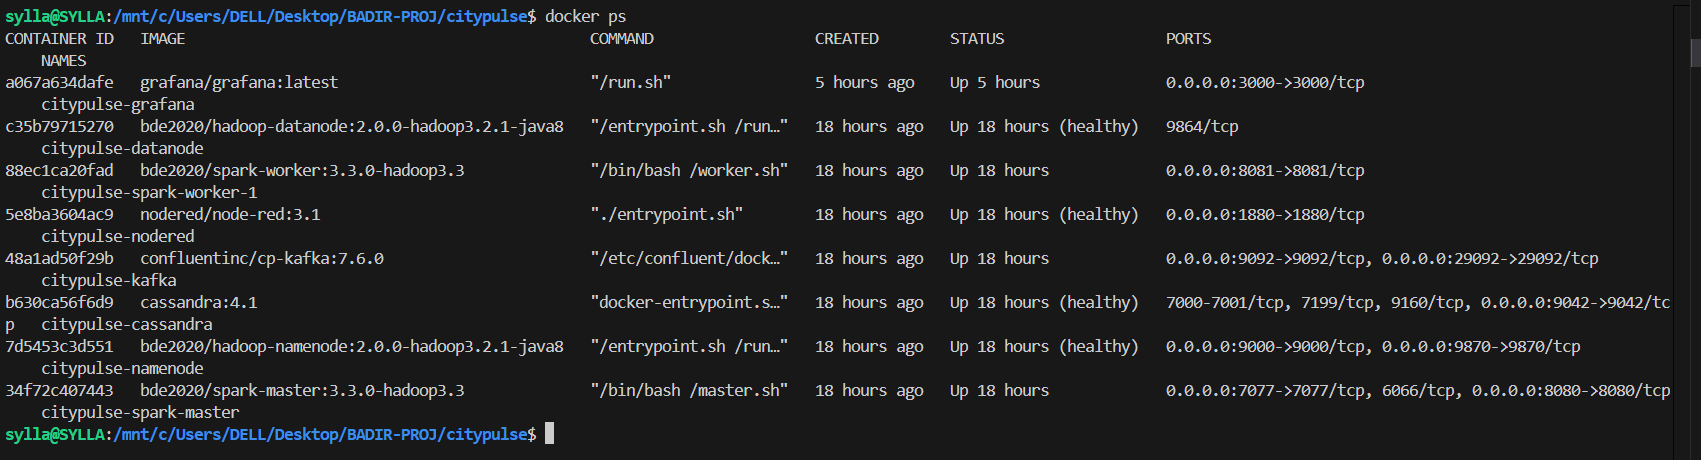
\includegraphics[width=\textwidth, height=4cm]{pictures/docker-ps.png}
    \caption{État des conteneurs via \texttt{docker ps} montrant l'infrastructure opérationnelle.}
    \label{fig:dockerps}
\end{figure}

\section{Sprint 2 : Silver Layer (Data Lake)}
Le script \texttt{SilverProcessing.scala} normalise les données. Nous utilisons l'API \textbf{Structured Streaming} de Spark.

Nous avons utilisé Node-RED pour simuler des capteurs. Le flux génère des JSON envoyés vers Kafka.

\begin{lstlisting}[language=Scala, caption=Nettoyage et écriture Parquet]
val cleanStream = rawStream
  .select(from_json($"value", schema).as("data"))
  .select("data.*")
  .withColumn("event_time", to_timestamp($"timestamp"))
  .writeStream
  .format("parquet")
  .option("path", "hdfs://namenode:9000/data/silver/traffic")
  .partitionBy("district")
  .start()
\end{lstlisting}

\begin{jointwork}
    \textbf{Solution :} Ajout d'un nœud \texttt{JSON Stringify} dans Node-RED avant le producteur Kafka.
\end{jointwork}

\begin{figure}[h]
    \centering
    % REMPLACEZ PAR VOTRE SCREENSHOT CONSOLE KAFKA
   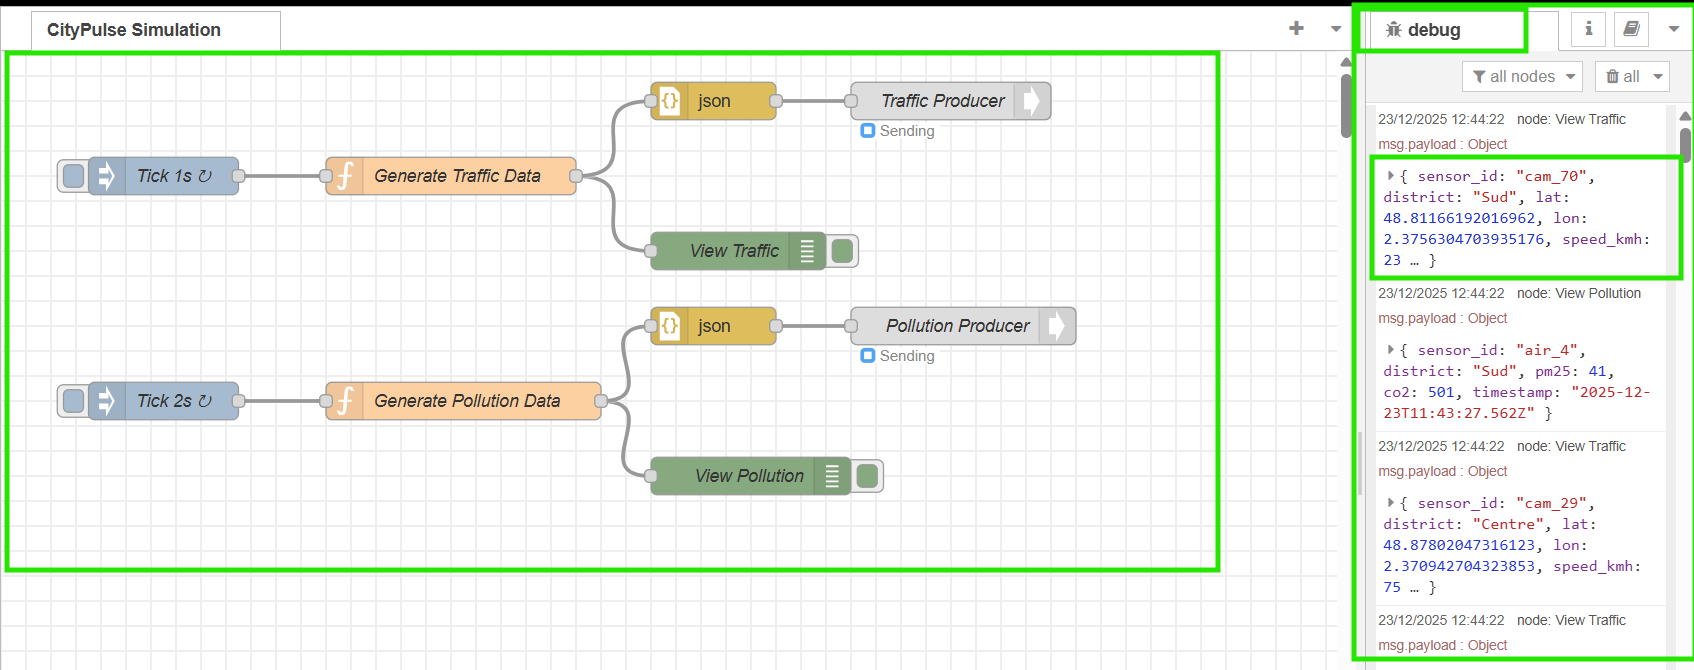
\includegraphics[width=0.9\textwidth]{pictures/node-red.png}
    \caption{Flux Node-RED de simulation.}
    \label{fig:nodered}
\end{figure}

Le résultat est visible dans la console du consommateur Kafka (\Cref{fig:kafka-console}).

\begin{figure}[h]
    \centering
    % REMPLACEZ PAR VOTRE SCREENSHOT CONSOLE KAFKA
    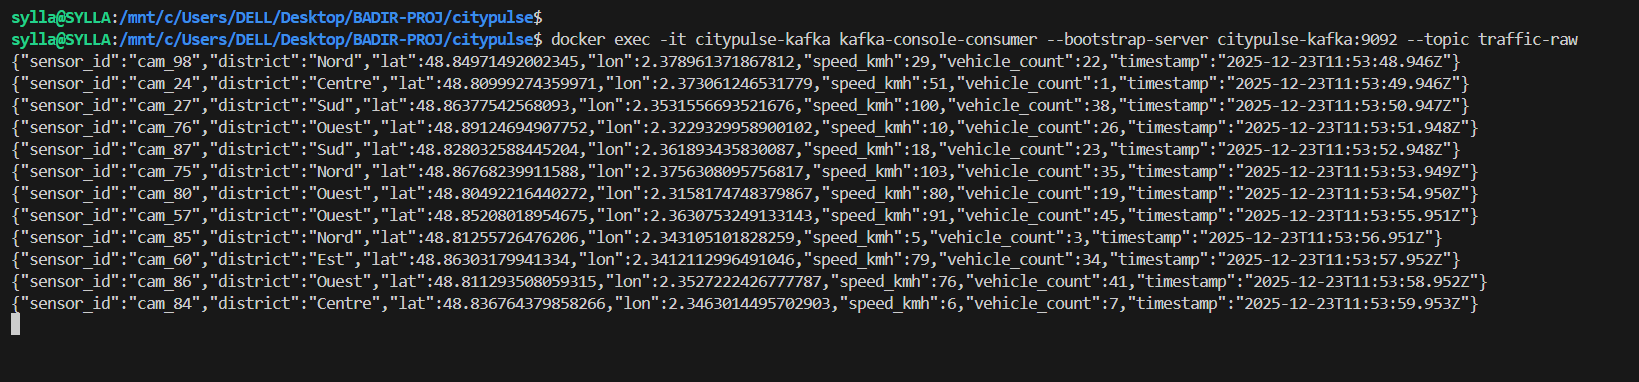
\includegraphics[width=0.9\textwidth]{pictures/kafkaconsole.png}
    \caption{Consommation des messages JSON dans la console Kafka.}
    \label{fig:kafka-console}
\end{figure}


\section{Sprint 3 : Gold Layer \& Streaming}

Le calcul des agrégats (moyenne par minute) a posé le problème des \textit{"Multiple streaming aggregations"}. Spark interdit de joindre deux flux agrégés dynamiquement.

\textbf{Solution technique :} Utilisation de la méthode \texttt{unionByName} pour fusionner les flux Trafic et Pollution avant d'effectuer une agrégation unique globale.

Le traitement Spark Structured Streaming constitue le cœur du système.

\subsection{Gestion des agrégations multiples}
Un défi technique majeur rencontré fut l'erreur \texttt{Multiple streaming aggregations not supported}. Pour contourner cela, nous avons unifié les flux avant l'agrégation.

\begin{lstlisting}[language=Scala, caption=Code Scala pour l'unification des flux et l'agrégation.]
// Fusion des flux pour eviter "Multiple Aggregations"
val unifiedStream = trafficRaw.unionByName(pollutionRaw)

val districtKPIs = unifiedStream
  .withWatermark("event_time", "1 minute") // Gestion des Late Data
  .groupBy(
    window(col("event_time"), "1 minute"),
    col("district")
  )
  .agg(
    avg("speed_kmh").as("avg_speed"),
    max("density").as("max_density"),
    avg("pm25").as("avg_pm25")
  )
\end{lstlisting}

\subsection{Logique d'alerte}
Les KPIs calculés sont ensuite enrichis avec une logique métier pour déterminer le niveau d'alerte (NORMAL, WARNING, CRITIQUE). Les résultats sont écrits dans Cassandra.

\begin{figure}[h]
    \centering
    % REMPLACEZ PAR VOTRE SCREENSHOT SPARK LOGS
    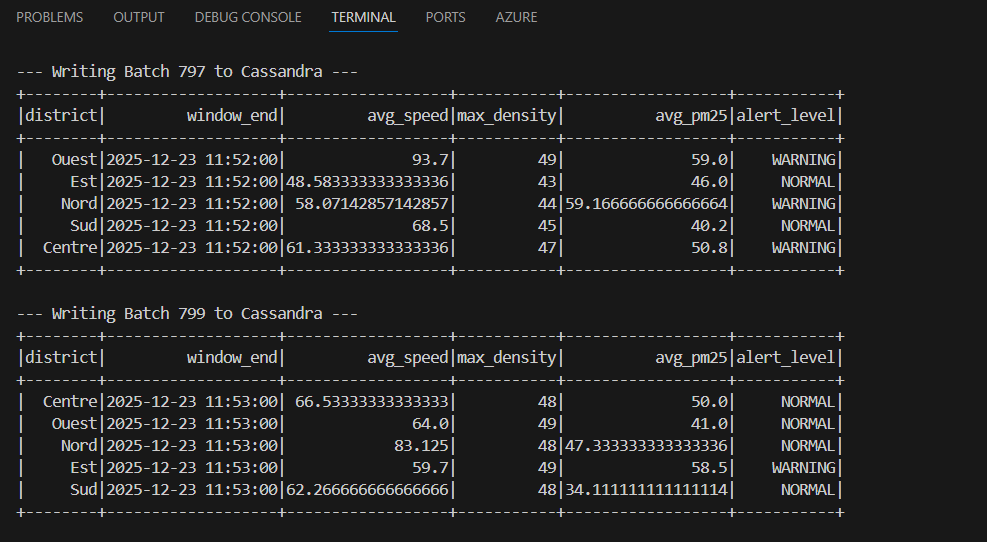
\includegraphics[width=\textwidth]{pictures/sparklog.png}
    \caption{Logs Spark indiquant l'écriture des micro-batchs vers Cassandra.}
    \label{fig:sparklogs}
\end{figure}

\section{Phase 4 : Visualisation (Grafana)}
Grafana interroge Cassandra pour afficher les métriques en temps réel. Le plugin \textit{HadesArchitect} a été utilisé pour la connexion.


\begin{figure}[h]
    \centering
    % REMPLACEZ PAR VOTRE SCREENSHOT CONSOLE KAFKA
    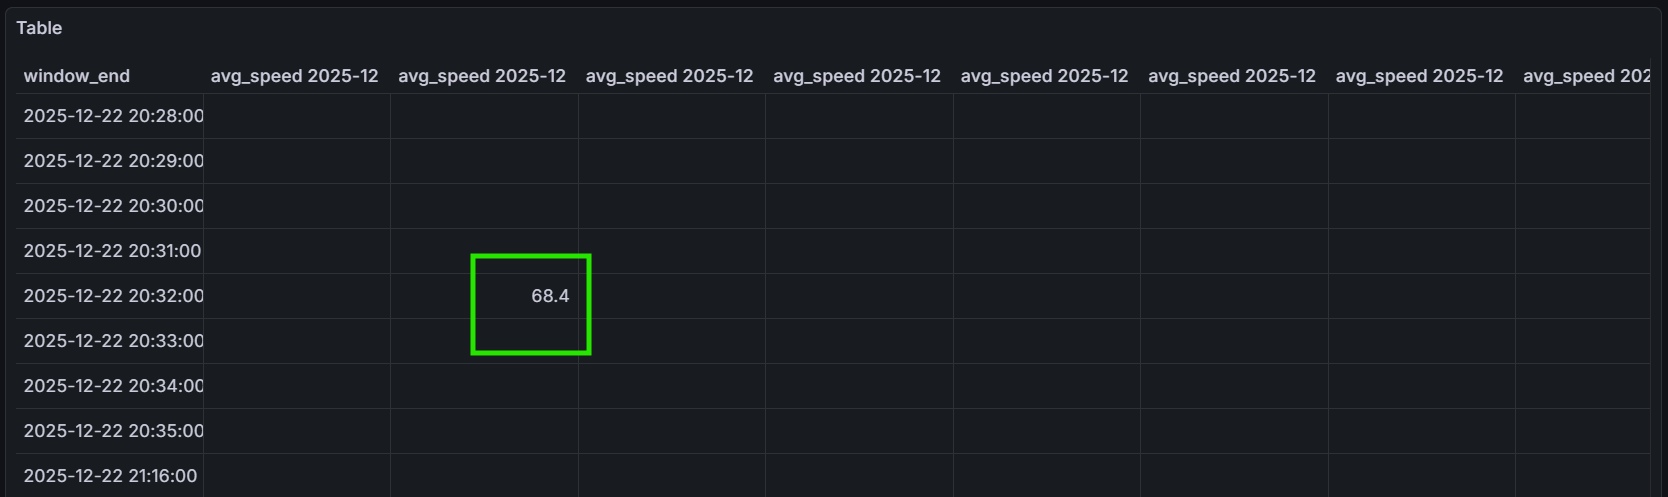
\includegraphics[width=\textwidth]{pictures/cqlsh.png}
        \caption{Données brutes dans Cassandra (cqlsh).}
        \label{fig:cassandra}
\end{figure}


\begin{figure}[h]
    \centering
    % REMPLACEZ PAR VOTRE SCREENSHOT CONSOLE KAFKA
    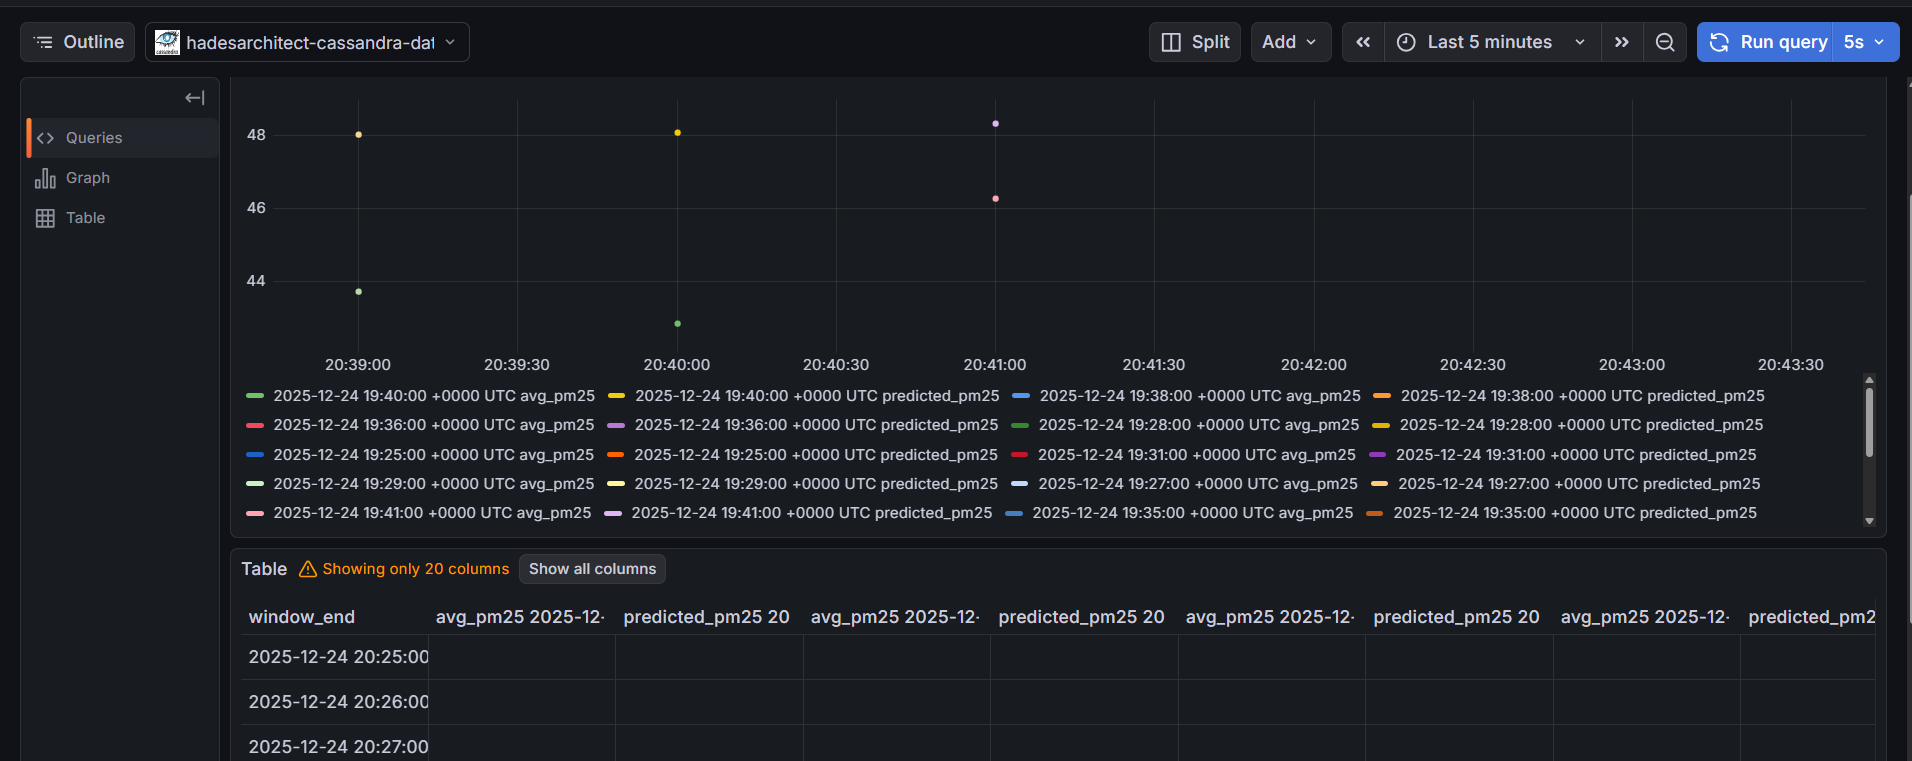
\includegraphics[width=\textwidth]{pictures/grafana.png}
        \caption{Dashboard Grafana final.}
        \label{fig:grafana}
   
\end{figure}


\section{Sprint 5 : Intégration du Machine Learning}
C'est la valeur ajoutée majeure du projet. Nous utilisons \textbf{Spark MLlib}.

\subsection{Entraînement (Offline)}
Le script \texttt{ModelTraining.scala} lit l'historique Parquet (Silver), joint les données de trafic et de pollution par heure, et entraîne une \textbf{Régression Linéaire}.
\begin{lstlisting}[language=Scala, caption=Entraînement du modèle]
val assembler = new VectorAssembler()
  .setInputCols(Array("speed_kmh", "vehicle_count"))
  .setOutputCol("features")
  
val lr = new LinearRegression().setLabelCol("pm25")
val model = new Pipeline().setStages(Array(assembler, lr)).fit(trainingData)

model.write.overwrite().save("hdfs://namenode:9000/models/pollution_v1")
\end{lstlisting}

\subsection{Inférence (Online)}
Le job de streaming charge ce modèle et l'applique à chaque micro-batch pour générer la colonne \texttt{predicted\_pm25}.

